%%%%%%%%%%%%%%%%%%%%%%%%%%  ltexpprt_twocolumn.tex  %%%%%%%%%%%%%%%%%%%%%%%%%%%%%%%%
%
% This is ltexpprt_twocolumn.tex, an example file for use with the SIAM LaTeX2E
% Preprint Series macros. It is designed to provide two-column output.
% Please take the time to read the following comments, as they document
% how to use these macros. This file can be composed and printed out for
% use as sample output.

% Any comments or questions regarding these macros should be directed to:
%
%                 Donna Witzleben
%                 SIAM
%                 3600 University City Science Center
%                 Philadelphia, PA 19104-2688
%                 USA
%                 Telephone: (215) 382-9800
%                 Fax: (215) 386-7999
%                 e-mail: witzleben@siam.org


% This file is to be used as an example for style only. It should not be read
% for content.

%%%%%%%%%%%%%%% PLEASE NOTE THE FOLLOWING STYLE RESTRICTIONS %%%%%%%%%%%%%%%

%%  1. There are no new tags.  Existing LaTeX tags have been formatted to match
%%     the Preprint series style.
%%
%%  2. Do not change the margins or page size!  Do not change from the default
%%     text font!
%%
%%  3. You must use \cite in the text to mark your reference citations and
%%     \bibitem in the listing of references at the end of your chapter. See
%%     the examples in the following file. If you are using BibTeX, please
%%     supply the bst file with the manuscript file.
%%
%%  4. This macro is set up for two levels of headings (\section and
%%     \subsection). The macro will automatically number the headings for you.
%%
%%  5. No running heads are to be used for this volume.
%%
%%  6. Theorems, Lemmas, Definitions, Equations, etc. are to be double numbered,
%%     indicating the section and the occurrence of that element
%%     within that section. (For example, the first theorem in the second
%%     section would be numbered 2.1. The macro will
%%     automatically do the numbering for you.
%%
%%  7. Figures and Tables must be single-numbered.
%%     Use existing LaTeX tags for these elements.
%%     Numbering will be done automatically.
%%
%%  8. Page numbering is no longer included in this macro.
%%     Pagination will be set by the program committee.
%%
%%
%%%%%%%%%%%%%%%%%%%%%%%%%%%%%%%%%%%%%%%%%%%%%%%%%%%%%%%%%%%%%%%%%%%%%%%%%%%%%%%


\documentclass[twoside,leqno,twocolumn]{article}
\PassOptionsToPackage{svgnames}{xcolor}

\usepackage{graphicx}
\usepackage{amsmath}
\usepackage{amssymb}
\usepackage{amsthm}
\usepackage{natbib}
\usepackage{xcolor}
\usepackage{hyperref}
\usepackage{xparse}
\usepackage{multirow}
\usepackage{float}
\usepackage{booktabs}
\usepackage[noend]{algorithm2e}
\usepackage{tikz}
\usepackage{appendix}
\usepackage{subcaption}
\usepackage{titling}
\definecolor{LightBlue}{HTML}{00F9DE}



\newtheorem{theorem}{Theorem}



\theoremstyle{definition}
\newtheorem{definition}{Definition}[section]





% Comment out the line below if using A4 paper size
\usepackage[letterpaper]{geometry}

\usepackage{ltexpprt}

\begin{document}

%
\newcommand\relatedversion{}
\renewcommand\relatedversion{\thanks{The full version of the paper can be
	accessed at \protect\url{FIXME}}} % Replace URL with link to full paper or comment out this line


%\setcounter{chapter}{2} % If you are doing your chapter as chapter one,
%\setcounter{section}{3} % comment these two lines out.

\title{\Large Visualizing Overlapping Biclusterings and Boolean Matrix
	Factorizations\relatedversion}
\author{Thibault Marette\thanks{ENS de Lyon, Lyon, France.}
\and Stefan Neumann\thanks{KTH Royal Institute of Technology, Stockholm, Sweden.}}

\date{}

\maketitle

% Copyright Statement
% When submitting your final paper to a SIAM proceedings, it is requested that you include
% the appropriate copyright in the footer of the paper.  The copyright added should be
% consistent with the copyright selected on the copyright form submitted with the paper.
% Please note that "20XX" should be changed to the year of the meeting.

% Default Copyright Statement
\fancyfoot[R]{\scriptsize{Copyright \textcopyright\ 20XX by SIAM\\
Unauthorized reproduction of this article is prohibited}}

% Depending on which copyright you agree to when you sign the copyright form, the copyright
% can be changed to one of the following after commenting out the default copyright statement
% above.

%\fancyfoot[R]{\scriptsize{Copyright \textcopyright\ 20XX\\
%Copyright for this paper is retained by authors}}

%\fancyfoot[R]{\scriptsize{Copyright \textcopyright\ 20XX\\
%Copyright retained by principal author's organization}}

%\pagenumbering{arabic}
%\setcounter{page}{1}%Leave this line commented out.

\begin{abstract} \small\baselineskip=9pt
Finding clusters in bipartite graphs is a popular problem in many communities such as data mining or bioinformatics. Drawing these clusters is simple as long as the clusters are disjoint but when the clusters share vertices then the task becomes more complicated.
We formalize the problem of drawing \emph{a given clustering} of overlapping clusters in bipartite graphs and we formulate an objective function that captures how well the clustering is visualized. We also present algorithms that optimize our objective function and we evaluate our methods on real-world datasets.
\end{abstract}





\section{Introduction}
\noindent In many data science tasks the goal is to understand the relationship of two different sets of entities. This problem is often modelled using bipartite graphs where the two sides of the bipartite graph correspond to the two sets of different entities. An edge indicates that two entities interact with each other (e.g., a customer has bought a product). Many (bi-)clustering algorithms try to find groups of related entities by finding dense subgraphs in the bipartite graph.

The development of algorithms for finding such clusterings has been an active research area for decades \cite{hartigan1972direct,asso,NEURIPS2018_ab731488}. However, these algorithms typically return their solutions in a format that is not human-readable. Therefore, inspecting the results can be difficult and visualization tools can be helpful.

Computing such a visualization is simple as long as all clusters are \emph{disjoint}, i.e., they do not share any vertices. However, when the clusters \emph{overlap}, i.e., some vertices are contained in multiple clusters, the visualization becomes more difficult~\cite{Vehlow2017VisualizingGS}. The main challenge is that, due to the overlap of the clusters, we might be forced to draw some clusters non-consecutively and the visualization needs to make a choice which clusters should be split up. Such overlapping clusters occur, for instance, in data mining~\cite{asso,BMFrecent} and in bioinformatics~\cite{1324618}.

In our work, we develop novel algorithms for drawing \emph{a given clustering} of a bipartite graph even when the clusters overlap. This is in contrast to seriation algorithms~\cite{MatrixReorderingSTAR,Xu2016InteractiveVC} which also allow us to find clusters in graphs but they cannot visualize a clustering that they obtain as input. Unlike many leaf-ordering approaches, we do not assume access to a (dis-)similarity function for the clusters or for the rows and columns of the input matrix; we elaborate on this below.

In our visualization we decide to draw the (bi-)adjacency matrix of the bipartite graph. Since the clusters represent dense subgraphs within the bipartite graph, each cluster induces a dense area of 1-entries in the adjacency matrix.
In Figure~\ref{fig:ord2} we visualize the outputs of two different clustering algorithms that were run on the \emph{same} dataset. The figure suggests that the left method finds smaller, denser clusters, whereas the right method finds larger, slightly sparser clusters. The left clustering in Figure~\ref{fig:ord2} also shows that some of the clusters have significant overlap (several columns appear in different row-clusters).

%We propose an algorithm that, given a bipartite graph and a clustering of the graph, finds a suitable visualization of the biadjacency matrix of the graph. Our approach is different from previous methods, which are unable to visualize a given graph clustering \cite{MatrixReorderingSTAR} \cite{Xu2016InteractiveVC}.

To obtain a good visualization of the clustering we need to reorder the rows and the columns of the biadjacency matrix based on the clustering.
We propose an objective function that generalizes to the overlapping setting and incentivizes orderings in which each cluster is drawn as a consecutive rectangle of 1-entries. When this is not possible, our objective function tries to maximize the squared area of the different non-consecutive parts of the clusters. We show that our objective function is NP-hard to optimize by proving that the associated decision problem: ``Can all clusters be drawn as a consecutive rectangle?'' is NP-complete via a reduction from MAX-Hamiltonian Path. %Then we show that the optimization problem enables us to solve the decision problem which yields the NP-hardness.

We also provide heuristics to optimize our objective function. To improve efficiency, we run a \emph{pre-processing step} that decomposes the overlapping clusters into disjoint \emph{blocks}. The blocks form a partition of the rows and columns of the matrix and each cluster corresponds to the union of a set of blocks. To obtain our visualization, it suffices to \emph{reorder the blocks}, as an ordering of the blocks implies an ordering of the rows and columns. Thus, the complexity of our ordering problem only depends on the number of blocks, which is small in practice. %$k$ different clusters can yield at most $2^k$ blocks, but this worst-case behavior is not reached in practice. This step reduces the time complexity of our algorithms by orders of magnitude.
In a \emph{post-processing step} we aim to improve the \emph{global} visualization; this is in contrast to our objective function which only \emph{locally} ensures that each clusters is drawn well individually. To ensure that the local structure of the visualization is not altered, we guarantee that we do not decrease the objective function.
An interesting question for future work is whether leaf-ordering methods such as \emph{dendosort}~\cite{Dendo} can be used to order the blocks that we create in the pre-processing. The main conceptual difference is that when drawing dendrograms, one has access to a function that measures the (dis-)similarity of a pair of clusters. However, in our setting we do not have such a similarity function for the blocks and proposing such a function seems like an interesting direction.


\section{Related Work}

\section{Preliminaries}
\noindent In order to define biclusters, we first define a biclique.

Given a bipartite gaph $G = (R \cup C,E)$, a \emph{biclique} in $G$ is a subgraph $B = (R'\cup C',E')$ such that $R' \subset R$, $C' \subset C$, and $E'=\{(r,c) \colon r\in R', c\in C'\}\subset E$.


\noindent In other words, $B$ is a biclique if and only if there is no edge between two elements of $R'$ or between two elements of $C'$, and there is an edge between all pairs of elements in $R' \times C'$. Consequently, the biadjacency matrix induced by $R'$ and $C'$ is a matrix of ones.

\medskip

\noindent There is no universal definition of a bicluster as it depends on the application. A good intuition nevertheless is to see them as ``incomplete bicliques'' (e.g. bicliques where some edges are missing), due to the fact that real-world data is not perfect. It can therefore also be viewed as a subgraph that has higher density than the full graph. Subsequently, for a bicluster $(R,C)$, we will denote the row related part of the cluster $R$ as \emph{row-cluster}, and the column related part $C$ as \emph{column-cluster}.

Due to its many applications, the task of finding biclusters in a bipartite graph has received a lot of attention. One way to tackle the problem is to see the biclustering problem as a Boolean Matrix Factorization (BMF) \cite{BMFrecent}. BMF is the Boolean variant of the matrix factorization problem: the goal is to find two smaller binary matrices such that their product is as close as possible as to the original matrix.

\medskip

\noindent Boolean Matrix Factorization (BMF):\\
Let $M \in \{0,1\}^{m\times n}$ and $k \in \mathbb{N}$ . The goal is to find two factor matrices $R \in \{0,1\}^{m \times k}$ and $C \in \{0,1\}^{k \times n}$ such that $||M - R \circ C||_2$ is minimized. Here, $\circ$ denotes the matrix-matrix multiplication in the Boolean algebra, that is to say, for all $i =1,...,m$ and $j=1,..,n$,
$$(R \circ C)_{ij} = \bigvee_{r=1}^k(R_{ir} \wedge C_{rj}).$$

\medskip

\noindent The link between BMF and biclustering becomes clear when we interpret the matrix $M$ as a biadjacency matrix. Indeed, the matrix product between row $i$ of $R$ and a column $i$ of $C$ yields an rank-1 matrix in which there is an edge between all elements of $R_i$ and $C_i$. Thus, $R_i \circ C_i$ corresponds to a biclique in the original graph, by definition. Consequently, if we have a BMF of $M$ with $R \in \{0,1\}^{m \times k}$ and $C \in \{0,1\}^{k \times n}$, then this corresponds to $k$ bicliques in the corresponding bipartite graph.


\section{Our Objective Function}

\begin{itemize}
	\item Define objective function (in a general way without resorting to blocks)
	\item Discuss ideas of objective function
\end{itemize}

\subsection{Computational Complexity.}

\noindent Let $n \in \mathbb{N}$. Let $[n]$ be the set of $n$ elements $\{1,...,n\}$, and for $i,j \in \mathbb{N}$, $i<j$, let

\begin{equation*}
    [i,j] =\begin{cases}
    (i,i+1,...,j-1,j) \text{ if } i<j\\
    (j,j+1,...,i-1,i) \text{otherwise}
    \end{cases}
\end{equation*}

\medskip


\noindent Let $l, \in \mathbb{N}$. Let $\mathcal{C} = \{C_1,...,C_n\}$ a set of $n$ elements. Let $\mathcal{B} = \{B_1,...,B_{l}\}$ such that for every $B \in \mathcal{B}$, $B\subseteq \mathcal{C}$. In other words, every element of $\mathcal{B}$ is a subset of elements of $\mathcal{C}$. In the rest of the paper, we suppose that every $B\in\mathcal{B}$ is distinct.

\begin{definition}
\textit{Perfect drawing of $C$}: \newline
We say that $C \in \mathcal{C}$ is perfectly drawn for a permutation $\pi:[l]\xrightarrow[]{} [l]$ if and only if for all pair $a,b \in [l]$, if $C \in B_{\pi(a)}$, and $C \in B_{\pi(b)}$, then for all $k \in [l]$, if $\pi(k) \in [\pi(a),\pi(b)] $, then $C \in B_k$.
\end{definition}
\noindent In other words, $C$ is perfectly drawn for a permutation $\pi$ if it appears in a consecutive fashion in the elements of the sequence $(B_{\pi(1)},...,B_{\pi(l)})$. 

\begin{definition}
Link to the Bicluster drawing problem: \newline
We treat each dimension (row/columns) independently. Indeed, a drawing of a biclustering is perfect if and only if the projection over the rows is perfect and the projection over the columns is perfect. \newline
Here, we have $n$ biclusters (the $n$ elements of $\mathcal{C}$). $\mathcal{B}$ is a partition of the rows (or the columns) of the matrix. Let $R_i$ be the $i$th element of the set of rows $\mathcal{R}$ of the matrix. A row will be identified by the clusters it belongs to. Hence, a row is a subset of $\mathcal{C}$. Then, we define $\mathcal{B}$ such that $\mathcal{B}$ is the smallest partition of $\mathcal{R}$ such that if $R_i \in B_k$ and $R_j \in B_k$, then $R_i = R_j$.
\end{definition}

\noindent The direct consequence of this is that if a bicluster is perfectly drawn over the rows and the columns, then it appears as a submatrix of ones in the original biadjacency matrix.

\begin{definition}
        \textit{PerfectOrdering} problem:\\
Given $\mathcal{C} = \{C_1,...,C_n\}$, and $\mathcal{B} = \{B_1,...,B_{l}\}$ such that for every $B \in \mathcal{B}$, $B\subseteq \mathcal{C}$, is there a permutation of these blocks, such that at least $k$ clusters are perfectly drawn with this permutation.
\end{definition}

\medskip

\noindent We will prove that \textit{PerfectOrdering} is equivalent to the NP-hard problem \textit{MAX Hamiltonian path}.


\begin{definition}
\textit{MAX Hamiltonian path}:\\
Given a weighted graph $G = (V,E,w)$ and a weight $W$, is there a Hamiltonian path $p$ such that  
$w(p) \geq W$ ?
\end{definition}



\medskip

\noindent We define for convenience w(p) to be $w(p) = \sum_{e\in p}w(e)$ .%, and $M = max_{x,y \in \mathcal{L}^2} w(x,y))$

\bigskip


\section*{Proof}

\subsection*{\textit{MAX Hamiltonian Path} $\xrightarrow[]{}$ \textit{PerfectOrdering Problem}}

\noindent Let $(\mathcal{C},\mathcal{B},k)$ be an instance of \textit{PerfectOrdering} problem. Consider the complete graph $G = (V, E, w)$ such that :
$V = \mathcal{B}$, and $for all B_i,B_j \in V$, $w(B_i,B_j) = |B_i \cap B_j|$

\bigskip


\noindent Let $p$ be an solution of $MAX Hamiltonian Path$ in $G$. let $\pi(i) = \text{order of apparition in }p\text{ of } B_i$ (the permutation is simply the order of appearance of $B_i$ in the path $p$).

\medskip

\begin{theorem}
When $C \in \mathcal{C}$ is perfectly drawn for permutation $\pi$, then the contribution of that cluster in the weight of the corresponding path in the graph is $|\{B_i, C \in B_i\}|-1$.
\end{theorem}

\begin{proof}

First, we formally define the notion of contribution of a cluster in the weight of the path in the graph. we know that $w(p)$ is the total weight of the path. However, we can partition the weight of the path over the contribution of each cluster of $\mathcal{C}$: $w(p) = \sum_{i=1}^{n}w_{i}(p)$, where $w_i(p)$ is the weight the path in the graph $G=(\{B_j \cap \{C_i\} , B_j \in \mathcal{B}\},E,w).$

\medskip

\noindent When $C$ is perfectly drawn for $\pi$, then by definition, there exists $a,b \in [n]$ such that for all $k \in [n]$, if $\pi(k) \in [\pi(a),\pi(b)]$, then $C \in B_k$. Since $C$ is perfectly drawn, we know $C$ appears in $B_{\pi(a)}, B_{\pi(a)+1},...,B_{\pi(b)}$. The contribution of $C$ in weight of the path in the graph is given by $w_i(p,\pi) = \sum_{i=0}^{n-1}(B_{\pi^{-1}(i)},B_{\pi^{-1}(i+1)}) = |\{B_i / C \in B_i\}|-1$
\end{proof}
 
 \bigskip
 
\noindent We want to solve our instance of \textit{PerfectOrdering} $(\mathcal{B},k)$. Then if there is a Hamiltonian path of weight at least $\sum_{i=1}^{k} |\{B_i / i \in B_i\}|-1$ in the graph discussed above, we get an ordering $\pi$ so that the $k$ biclusters are perfectly drawn. Otherwise, we know that there is no such ordering.


\subsection*{\textit{PerfectOrdering Problem} $\xrightarrow[]{}$ \textit{MAX Hamiltonian Path}}

We have an instance of Hamiltonian, for a graph $G = (\mathcal{V},E,w)$, and we wish to known whether it exists a path of weight at most $W$.

\noindent To do so, we build an instance of \textit{PerfectOrdering} such that:
\begin{itemize}
    \item $n=\sum_{e\in E}w(e)$
    \item For every $v\in \mathcal{V}$, we create $B_v \in \mathcal{B}$ such that for every $B_v \in \mathcal{B}$, $|B| = \sum_{u\in \mathcal{V}}w(u,v)$, for every $B_v, B_u \in \mathcal{B}$, $|B_v \cap B_u| = w(B_u,B_v)$, and for all $B_t, B_u, B_v \in \mathcal{B}, B_t \cap B_v \cap B_u = \emptyset$. The two last conditions ensures that the biclusters appear in exactly two different $B_v$. Indeed, if a bicluster appears in 3 or more different $B_v$, then it contradicts the last property. If a bicluster appears in exactly one $B_v$, then we have in the end more than $n$ biclusters.
\end{itemize}
\noindent Let's assume we have an ordering $\pi$ such that $W$ biclusters are perfectly drawn. Then, the path $p = (B_{\pi(1},...,B_{\pi(l})$ has the weight $w(p) = \sum_{i=1}^{l-1}w(B_{\pi(i},B_{\pi(i+1}) =  \sum_{i=1}^{l-1}|B_{\pi(i} \cap B_{\pi(i+1}|$. Each bicluster appear in exactly two biclusters, and since $W$ are perfectly drawn with the permutation $\pi$, then we have an upper bound such that $w(p) \geq W$.

\section{The Algorithm}
\noindent In the general case, the biclustering algorithms will output semi-complex or complex biclustering. Thus, Algorithm \ref{algoPerfect} is typically not satisfactory to draw biclusters. In the rest of the section, we assume that there exist biclusters that share elements such that the drawing is not trivial. In the rest of this section, we will describe how the algorithm works. An overview of the algorithm is shown in Figure \ref{fig:overview}. In this section, we start by describing the pre-processing step.

\begin{figure}
    \centering
    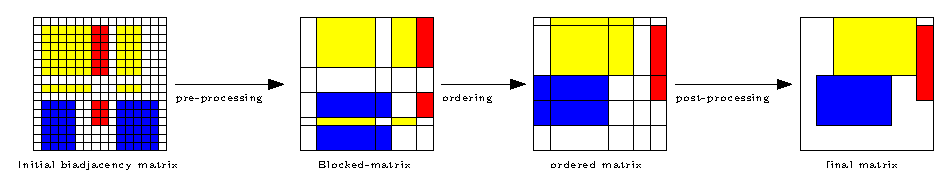
\includegraphics[width=\textwidth]{figures/algorithmOverview.eps}
    \caption{Overview of the bicluster visualization algorithm. The tiles in white corresponds to '0' elements, and the tiles in colour to '1' elements. Tiles that share the same colours belong to the same bicluster.}
    \label{fig:overview}
\end{figure}


\subsection{Pre-Processing.}
\noindent First, note that finding the best permutation over the rows and columns of a matrix of size $m\times n$ is a difficult task since there are $m!n!$ different pairs of row and column permutations. We can reduce this number as many of the visualizations are isomorphic (e.g., mirroring the
matrix vertically or horizontally does not change the visualization) although the
permutations are not the same. Still, even the number of different patterns is too high to compute an exact solution \cite{nphard}.


\medskip

\noindent Since the goal of the algorithm is to draw the biclusters as good as possible, we \emph{group together} the rows or columns that belong to the same clusters. To do so, we use the definition of a minimum block partitioning. In this report $[n]$ denotes the set of integers from $0$ to $n-1$.

\medskip
\begin{definition}
\label{def:blocks}
Let $\mathcal{L} = \{L_1,...,L_k\}$ be subsets of a set $[n]$. We say that $B_1,...,B_r$ is a \emph{block partitioning of $\mathcal{L}$ with $r$ blocks} if:
\begin{itemize}
\item  $B_j \subseteq [n]$ for all $j \in [r]$,
\item $\bigcup_{j \in [r]} B_j = [n]$,
\item $B_i \cap B_j = \emptyset$ for all $i \neq j$,
\item for all $i \in [k]$, there exists a set of indices $J \subseteq [r]$ such that $L_i = \bigcup_{j \in J} B_j$.
\end{itemize}

 We say that $B_1,...,B_r$ is a \emph{minimum block partitioning for $\mathcal{L}$} if there exists no block partitioning of $\mathcal{L}$ with $r-1$ blocks.
\end{definition}

\noindent Subsequently, we will denote the $B_j$ of Definition \ref{def:blocks} as \emph{blocks}. In practice, we will use the minimum block partitioning in order to aggregate the row-elements and column-elements of the adjacency matrix. In that case, to retrieve the row partitioning (resp. the column partitioning), the $[n]$ of Definition \ref{def:blocks} is the set of rows (resp. columns), and $\mathcal{L}$ is the set of row-clusters (resp. column-clusters). Thus, after the pre-processing, we computed $r$ blocks $B_1,...,B_r$ such that each block regroup all rows (or columns) that belong to the same set of clusters. An algorithmic description of the blocks is available in Algorithm \ref{algo:blockCreation} in  Appendix \ref{appendix:blocks}

\medskip

\noindent Thanks to the pre-processing step, we do not need to reorder the rows and columns of the matrix explicitly, but rather the blocks of rows and blocks of columns of the matrix. Thus, the ordering step will output a block ordering. The final ordering of all elements of the matrix is given by the order in which the elements appear in the block ordering. Note that since all rows and columns are contained in exactly one block, this implies an ordering of the rows and columns. Furthermore, due to how the blocks are grouped together, the final ordering should also be of better quality. Indeed, all rows (or columns) that belong exactly to the same clusters will be consecutive in the final picture, which is desirable.


\subsection{Computing the Block Ordering.}
The second step in designing our algorithm is to define an objective function, in order to have a numerical value to quantify how well the permutations draw the biclustering. There are several considerations that lead to the design of the objective function in this section.

\medskip

\noindent \sloppy First, the objective value of two biclusters should be independent from one to another. That is to say that if we seek to draw biclusters $A$ and $B$, then the score of bicluster $A$ should not have any influence over the score of bicluster $B$. Of course, if cluster $A$ and $B$ overlap, then their score will be linked implicitly. We denote $P_R$ the set of all permutations over the elements of $R$, and $P_C$ the set of all permutations over the elements of $C$. Thus, we consider $S:(2^{|R|}\times 2^{|C|})\times (P_R\times P_C)\xrightarrow[]{}\mathbb{R}_+$ a \emph{score function} given to a single bicluster for a specific permutation of rows and columns. The golbal objective function will be referred as \textit{MaximizeClusterArea} in the rest of the report.


\bigskip

\noindent Now, the score function is chosen according to how we want to represent the cluster. As biclusters represent elements that have high interaction with each other, the objective is to have all the components of the bicluster drawn together as closely as possible. We define the score of a cluster by

$$
S(R,C) = \sum_{\text{rect}\in \mathcal{R}(R,C)} \operatorname{area}(\operatorname{rect})^2.
$$

\medskip

\noindent  Here, $\mathcal{R}(R,C)$ is the set of rectangles that compose the bicluster $(R,C)$.
\begin{definition}
\label{def:rect}
Let $L$ be subsets of a set $[n]$. We say that $R_1,...,R_r$ is a \emph{rectangle partitioning $L$ with $r$ edges} if:
\begin{itemize}
\item  $R_j \subseteq [n]$ for all $j \in [r]$,
\item $\bigcup_{j \in [r]} R_j = L$,
\item $R_i \cap R_j = \emptyset$ for all $i \neq j$,
\item for all $l \in [r]$, for all $i,j \in R_l$, there exists a sequence of elements of $R_l$ $r_1,...,r_f$ such that $r_1=i$, $r_f=j$, and $r_k=r_{k+1}+1$ for all $k=1,...,f$.
\end{itemize}
\end{definition}

 \noindent We say that $R_1,...,R_r$ is a \emph{minimum rectangle partitioning for $L$} if there exists no block partitioning of $L$ with $l-1$ blocks. Subsequently, we will denote $\operatorname{CSQ}$ the function that returns the minimum rectangle partitioning of any given $L$.

 \medskip
 \noindent Then, we can define $\mathcal{R}$ such that $\mathcal{R}(R,C) = \operatorname{CSQ}(R) \times \operatorname{CSQ}(C)$, where $\times$ is the Cartesian product.

 \medskip

 \noindent Finally, we can define $\operatorname{area}$, which is $\operatorname{area}(rect)=\operatorname{area}(L_r,C_r) = \operatorname{size}(L_r)\cdot \operatorname{size}(C_r)$.


In Figure \ref{fig:clusterArea}, a biadjacency matrix is depicted in red, where $R=[1,2,4]$ and $C=[1,3,5]$. Then we have by definition $\operatorname{CSQ}(R) =[1,2],[4]$ and $CSQ(L) = [1],[3],[5])$. Thus, this gives us 6 rectangles : $([1,2],[4]) \times ([1],[3],[5])$. We can finally compute the score of that bicluster: $S(([1,2],[4]) \times ([1],[3],[5]))= 2 + 2 + 2 + 1 + 1 + 1 = 9.$
\begin{figure}
    \centering
    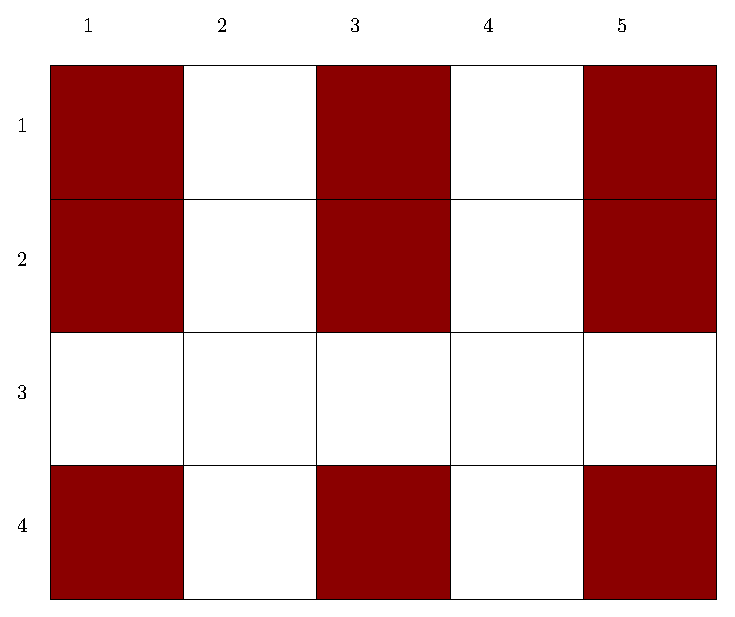
\includegraphics[width=0.33\textwidth]{figures/clusterArea.eps}
    \caption{Example of an adjacency matrix depicting a bicluster (in red). We can notice that the bicluster is in 6 different connected blocks, referred to as \emph{rectangles}.}
    \label{fig:clusterArea}
\end{figure}
\medskip

\noindent We can notice that $S(R,C)$ is only maximized when the biclusters $(R,C)$ is drawn as one connected component (i.e. all elements of R and C are consecutive in the ordering), which is exactly what we wanted based on our intuition.

\medskip

\noindent The global objective function \textit{MaximizeClusterArea} is

$$
\max _{\pi_R, \pi_C} \sum_{i=0}^{k}S((R_i,C_i),(\pi_R,\pi_C)).
$$

\noindent  We chose a sum function to aggregate the score of all biclusters, as it captures the idea that we evaluate the quality of the drawing of each cluster independently.

\noindent The objective function from Section \ref{objectiveFunction} leaves us with a permutation optimization problem. Exact algorithms such as dynamic programming or branch and bound are not suitable for this problem as the size of the matrices, even after the elements have been grouped by blocks, remains too large \cite{hahsler2008getting}. In recent years, a plethora of meta-heuristics search have been developed, such Multi-start
Local Search \cite{localSearch}, Simulated Annealing \cite{SA}, Tabu Search \cite{tabu} and Genetic Algorithms (GAs)
 \cite{optimizationbook}.

\medskip

\noindent  We settled on a specific kind of Genetic Algorithm that is specialized for permutation problems developed by Wang and Wu \cite{Wang2004HybridGA}. The general idea of GAs to solve an optimization problem is to initialize a population of solutions, and iteratively explore new solutions, by performing operations on the current population. These operations are crossovers (mix of two solutions from the population), and mutations (transformation of a solution by itself). To solve \emph{permutation} optimization problem with GAs, the population of the GA is made of the permutations. The particularity of the chosen GA is that it has a learning component by using a Neighbour Search (NS). We will refer to this technique as Hybrid Genetic Algorithm (HGA), and it is thoroughly described in \cite{Wang2004HybridGA}.

 \medskip

 \noindent The idea of the HGA is to merge the advantages of GAs and NS: while GAs are good at global search but poor at convergence, NS is good at fine-tuning but poor at finding global optima. The general behaviour of the algorithm can be seen in Figure \ref{fig:hga} in Appendix \ref{appendix:algorithms}.


 \medskip

\noindent The pseudo-code of the algorithm is described in \cite{Wang2004HybridGA}. Basically, there is the 'classical' genetic algorithm component, that is the initialization and the cycle fitness evaluation - parent selection - crossover - mutation - replacement. Each of these operation is chosen carefully to be suitable to a permutation optimization problem. Then, the learning part is added, after the initialization step and after each mutation step. The learning operation is a NS, performed over every permutation in the population.

\medskip

\noindent Here, the NS is done through a local search. The idea is that, given a state of the optimization problem, we visit iteratively all the neighbour of that state in order to refine the solution. In this case, a state of the optimization problem is a permutation, and the neighbour states are all permutations that can be obtained with a switch of two elements in the permutation. The local search stops when there is no neighbour that can increase the score. Of course, in this algorithm, we do not perform a full local search at each learning step, as it would precipitate the algorithm into local optima. Instead, only one step of local search is done at each learning step.


\subsection{Post-Processing.}

The post-processing is a step to improve the final drawing. The goal of this step is to have a better score from a seriation point of view (a better image globally), without hindering the quality of the bicluster drawing. Indeed, the objective function described in Section \ref{objectiveFunction} only values how well the biclusters are drawn, and not the quality of the \emph{global} picture, which can be insufficient for some applications. For instance, consider two biclusters $(L_1,R_1)$ and $(L_2,R_2)$. If the clustering outputs two non-overlapping yet very similar clusters (e.g. $R_1 \cap R_2 = \emptyset$ and $|C_1 \cap C_2| \simeq |C_1 \cup C_2|$), that could have be interpreted as one big cluster by the analyst and it is desirable that the two clusters are drawn nearby (i.e. $R_1$ and $R_2$ are close in the ordering). This is particularly helpful if a clustering algorithm outputs biclusters that do not overlap over rows (like PCV).

\medskip

\noindent Figure \ref{fig:postProcessing} shows the issue. On the left biadjacency matrix is depicted an ordering such that all biclusters are perfectly drawn. However, the biadjacency matrix on the right side has a better final ordering, despite having the same \textit{MaximizeClusterArea} objective function value.

\begin{figure}[t]
    \centering
    \begin{minipage}{0.45\textwidth}
        \centering
        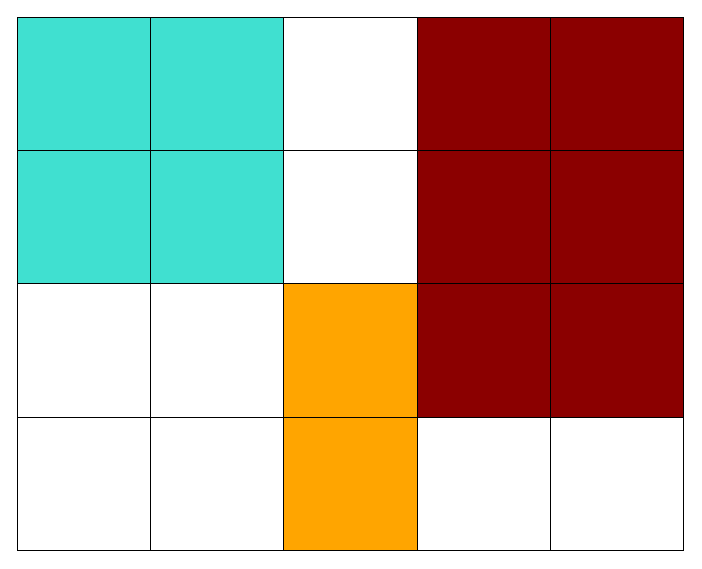
\includegraphics[width=0.6\textwidth,angle=90]{figures/perfectClustering.eps} % second figure itself
    \end{minipage}\hfill
    \begin{minipage}{0.45\textwidth}
        \centering
        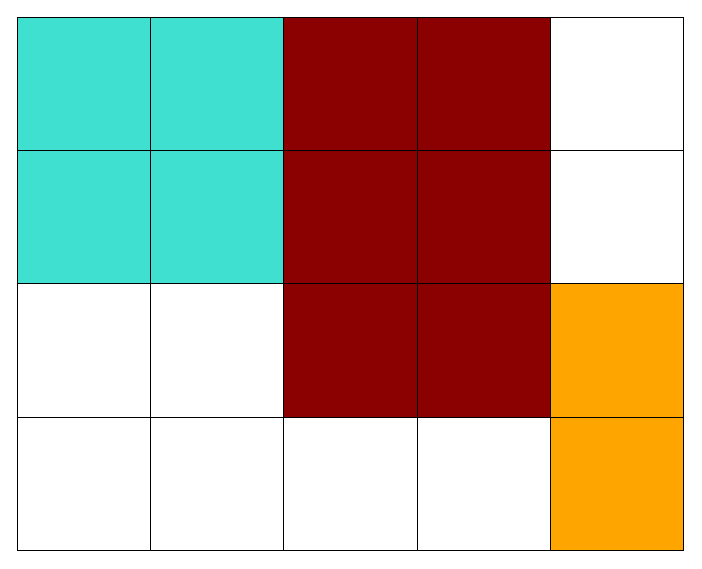
\includegraphics[width=0.6\textwidth, angle=90]{figures/perfectSeriation.eps} % first figure itself
    \end{minipage}
    \caption{The effect of post-processing over a biadjacency matrix. There are three clusters represented in these pictures, each cluster is drawn using a different colour. The left matrix is the result after the ordering step. The right matrix is the result after the post-processing step.}
    \label{fig:postProcessing}
\end{figure}

\bigskip

\noindent In order to increase the seriation score without lowering the \textit{MaximizeClusterArea} score, we build groups of blocks (that we will name \textit{connected blocks}), so that permuting two groups of blocks does not lower the \textit{MaximizaClusterArea} objective function. Thus, two neighbour blocks belong to the same connected block if they have at least one bicluster in common.
\medskip

\begin{definition}
\label{def:connectedblocks}
Let $\mathcal{B} = \{B_1,...,B_r\}$ and $\mathcal{C} = \{C_1,...,C_k\}$ be subsets of a set $[n]$, and $\pi:[r]\xrightarrow[]{}[r]$ an ordering of $\mathcal{B}$. Let  We say that $A_1,...,A_l$ is \emph{connected block partitioning of $\mathcal{B}$ with $l$ blocks} if:
\begin{itemize}
\item  $A_j \subseteq \mathcal{B}$ for all $j \in [r]$,
\item $\bigcup_{j \in [l]} A_j = \mathcal{B}$,
\item $A_i \cap A_j = \emptyset$ for all $i \neq j$,
\item for all $a \in [l]$, for all $B_i,B_j$ in $A_a$, $i\neq j$, if $\pi(i) = \pi(j)+1$, then $B_i \cap B_j \neq \emptyset$
\end{itemize}
 We say that $A_1,...,A_l$ is a \emph{minimum connected block partitioning for $\mathcal{B}$} if there exists no block partitioning of $\mathcal{B}$ with $l-1$ blocks.
\end{definition}


\medskip

\noindent We refer to $A_1,...,A_l$ of Definition \ref{def:connectedblocks} as \emph{connected blocks}. In that case, $\mathcal{B}$ is the set of blocks and $\mathcal{C}$ the set of biclusters. Once the connected blocks are built, we are left with a problem similar to the seriation problem, as we wish to rearrange the connected blocks and connected rows based on some similarity criterion. As for the pre-processing, the final ordering of the matrix is induced by the ordering of the connected blocks. Indeed, as all blocks belong to the connected blocks, an ordering of the connected blocks gives an ordering of the blocks, based on the order in which the blocks appear in the connected blocks ordering. Then, as before, the ordering of the blocks yields the ordering of the final matrix. %The difference however is that connected blocks are built by merging neighbour blocks, and these blocks might represent different biclusters. Thus, the first and last element of the connected block are not necessarily similar column. 

\section{Experiments}

\subsection{Datasets, Clustering and Visualization Algorithms.}
\begin{itemize}
	\item Description of the datasets we use.
	\item As baselines we should use: Dhillon~\cite{dhillon01coclustering},
		basso, message passing and some seriation methods (see below).
	\item Brief introduction of the visualization algorithms that we use.
\end{itemize}

\subsection{Measuring the Quality of the Visualizations.}
\begin{itemize}
	\item Define the objective functions of seriation and other measures that we
		need.
\end{itemize}

\subsection{Evaluation on Synthetic Data.}
\begin{itemize}
	\item Synthetically generate some data and visualize the results. This
		should include data on which the algorithms perfectly recover the
		ground-truth and also data on which the algorithms do not work
		perfectly.
	\item Discuss what happens when we do not run the pre-processing or the
		post-processing.  Discuss different algorithms for computing the block
		orderings.
\end{itemize}

\subsection{Comparison With Seriation Algorithms.}
\begin{itemize}
	\item Should be done on real-world data.
	\item We check which seriation scores are returned by our algorithms and
		competitors. (Perhaps also other measures?)
	\item Compare against: (1)~The slow local search algorithm we already have.
		(2)~A faster version of the local search algorithm which stops when the
			decrease of the objective function is less than $0.5\%$ (or so).
		(3)~Some other method for seriation that is popular in the seriation
			literature.
\end{itemize}

\subsection{Case Study: Visualizing Algorithm Results.}
\begin{itemize}
	\item Should be done on real-world data.
	\item Compare the clustering results of the different clustering algorithms.
\end{itemize}

\section{Conclusion}

\section{Other Tasks}
\begin{itemize}
	\item Clean up the code such that it has some documentation and such that
		there is a clean interface to use the code.
\end{itemize}

\bibliographystyle{plain} 
\bibliography{main}
\bibliography{referencesAbstract}
\bibliography{references}

\end{document}

% End of ltexpprt.tex 
